

\subsection{One-to-one}

Here we have two curves given by hand-annotation of the Romer
dataset. We build a grammar from the curve on the left, using a
hand-built set of constituents. We then parse the curve on the right,
and show the Viterbi parse by showing the correspondences between the
two curves.

Because there are no missing or extra points, this is straightforward.

%% we can use \input{} here to incorporate dynamically generated text

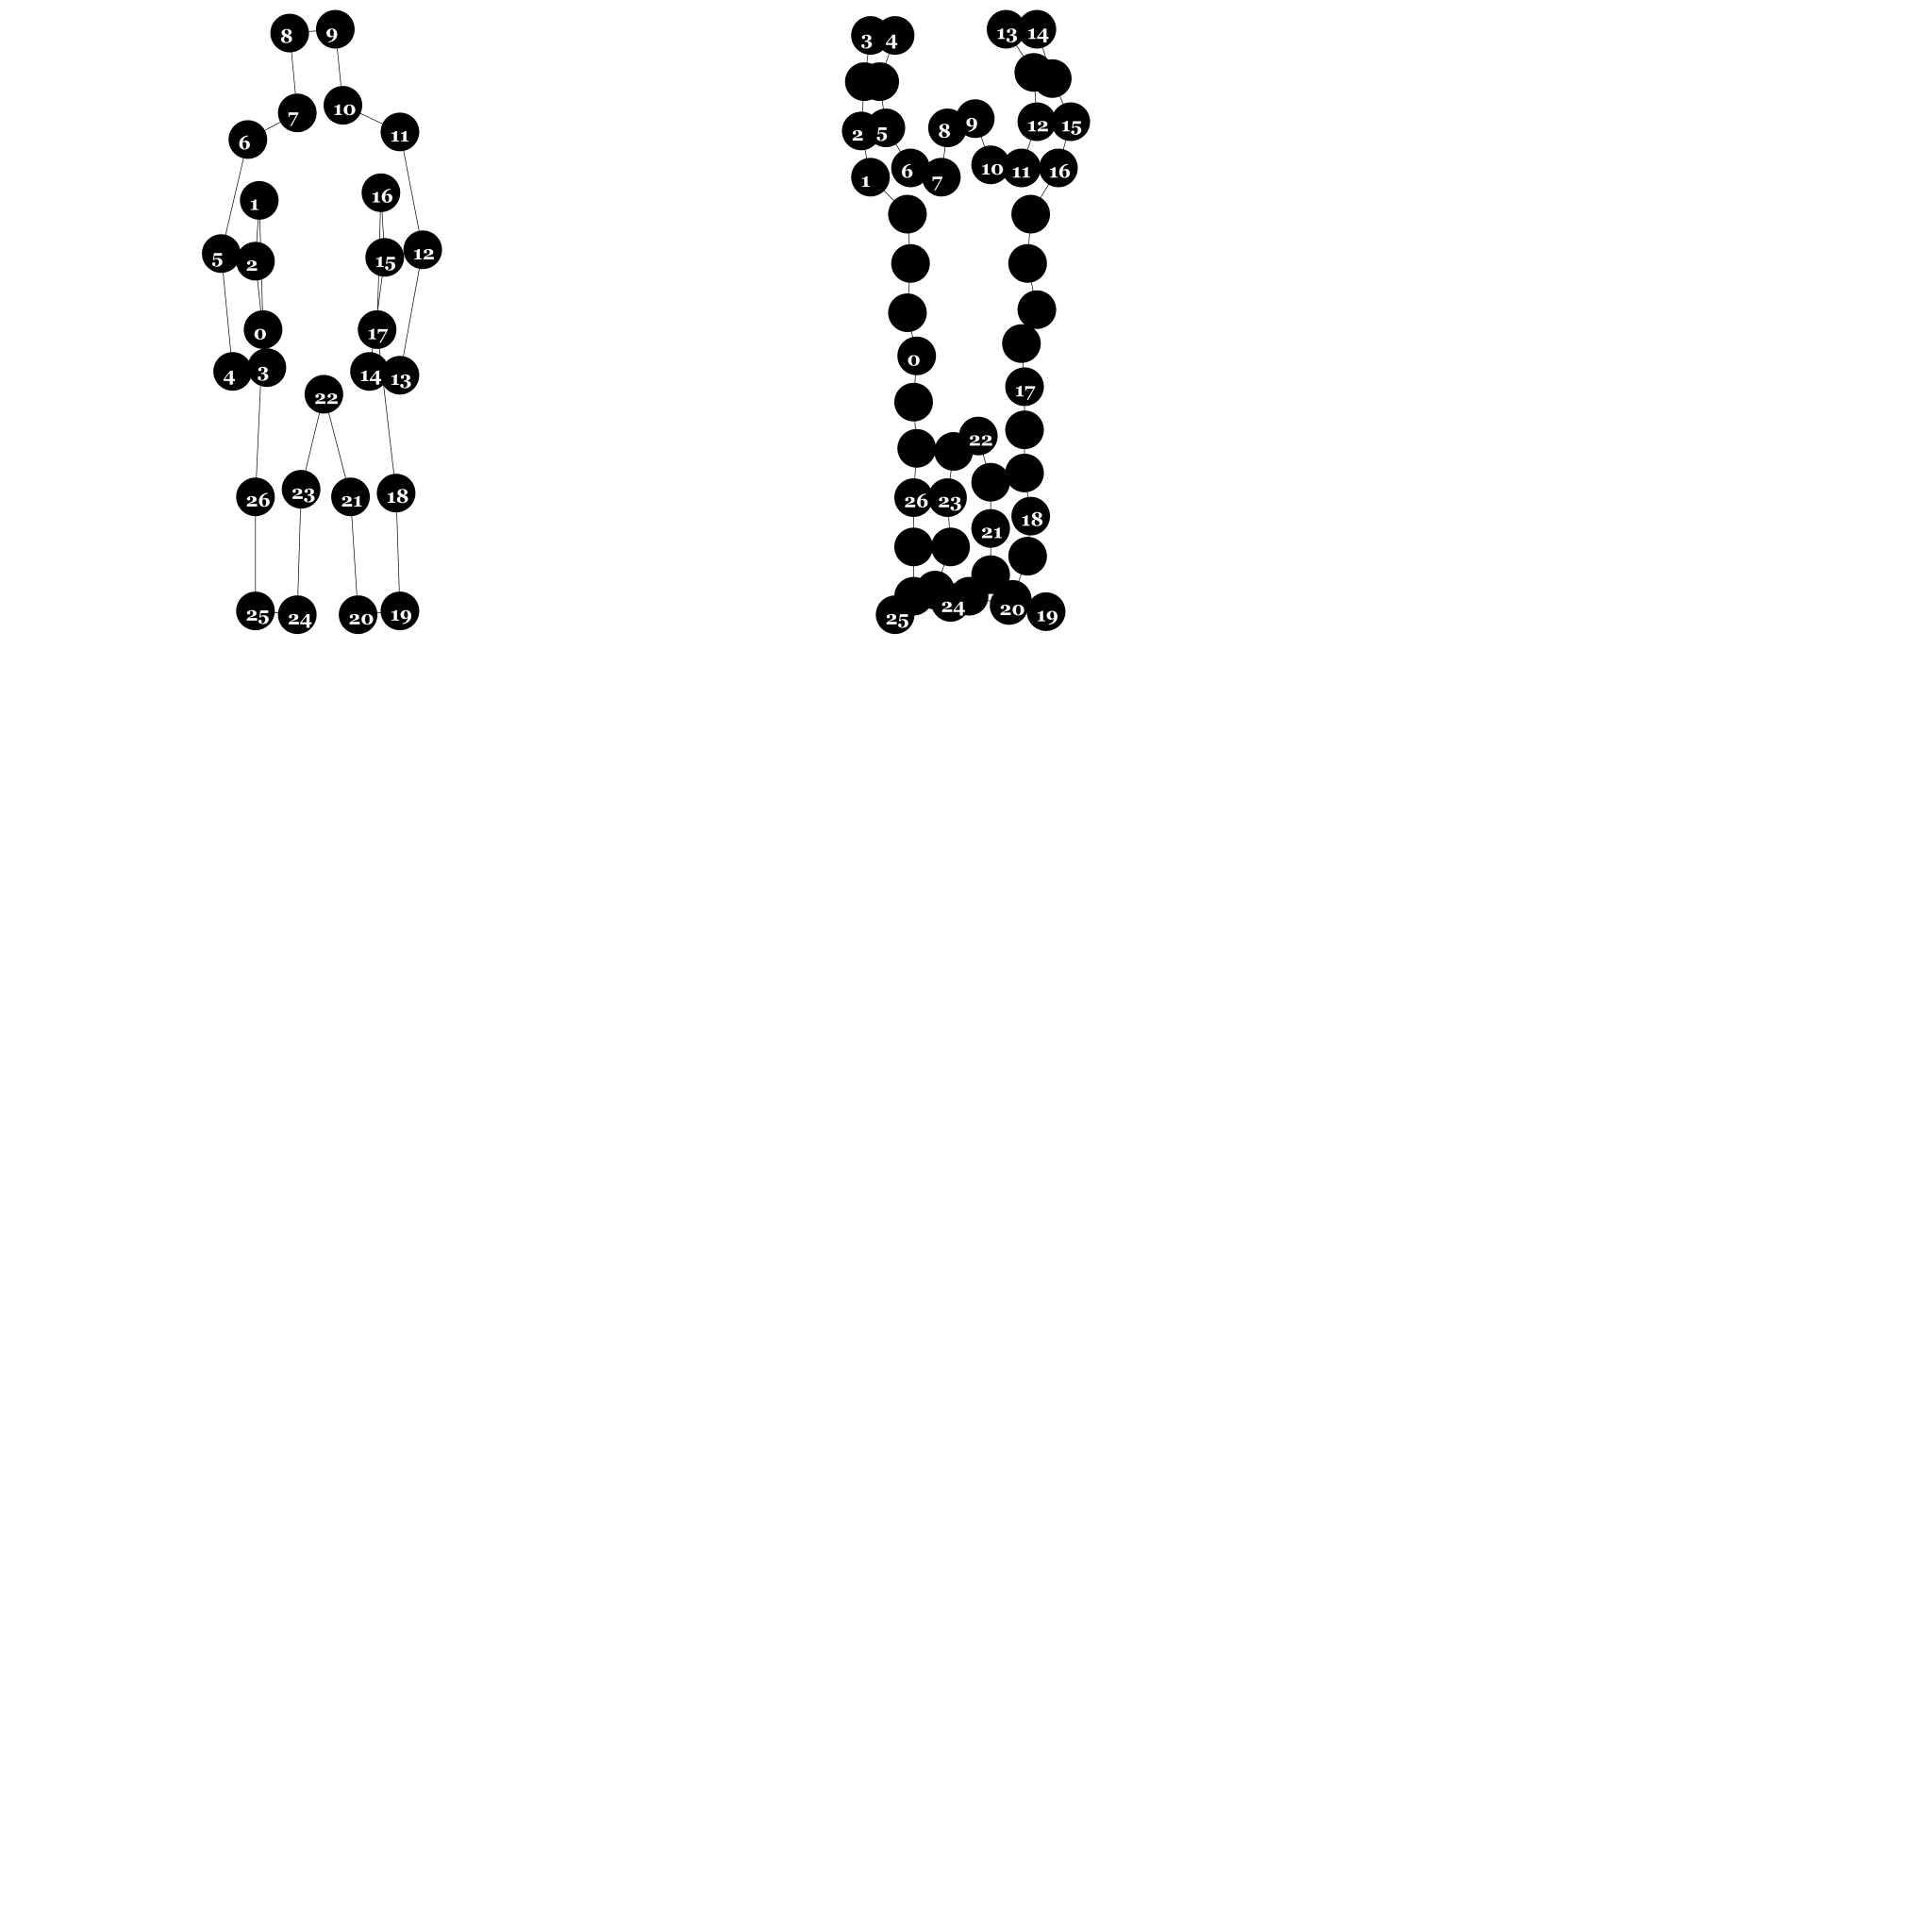
\includegraphics[width=6in]{./2.parsing/one_to_one/parse.eps}

